\documentclass{article}
\usepackage{tikz}
\usetikzlibrary{shapes,through,intersections,calc}
\usepackage{xcolor}
\begin{document}
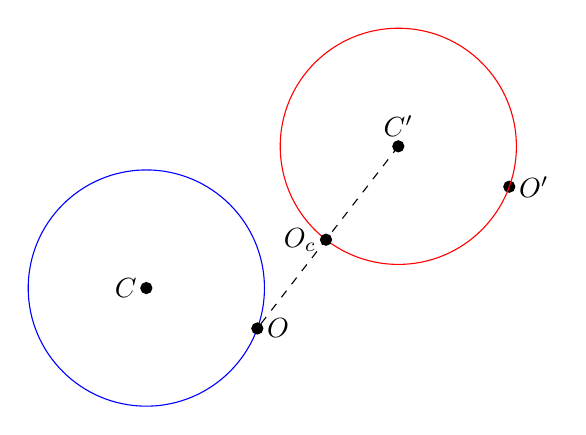
\begin{tikzpicture}
    \coordinate (P) at (0,0);
    \coordinate (Q) at (-20:15mm);
    \draw[blue] (P) circle (15mm);
    \draw[fill] (P) circle (2pt);
    \draw[fill] (Q) circle (2pt);
    \node at (P) [left]{$C$};
    \node at (Q) [right]{$O$};
    \begin{scope}[xshift=32mm, yshift=18mm]
        \coordinate (P1) at (0,0);
        \coordinate (Q1) at (-20:15mm);
        \node at (P1) [above]{$C'$};
        \node at (Q1) [right]{$O'$};
        \draw[fill] (P1) circle (2pt);
        \draw[fill] (Q1) circle (2pt);
        \node(c) at (P1) [draw,red,circle through=(Q1)] {};
        \coordinate(Q2) at (intersection 1 of c and P1--Q);
        \draw[fill] (Q2) circle (2pt);
        \node at (Q2) [above,left]{$O_c$};
    \end{scope}
    \draw[dashed] (P1) -- (Q);
\end{tikzpicture}

\section*{Moving Circles}

The \textcolor{blue}{blue} circle is \textbf{before} move and the
\textcolor{red}{red} circle is \textbf{after} move.
$O_c$ is the point on the red circle closest to $O$.

\subsection*{Using Plane Geometry}

To keep the outer point $O'$ on the red sphere as close as possible to its original position $O$ before the move.
\begin{itemize}
    \item Rotate $O'$ around $C'$ into $O_c$
    \item $O_c$ is a point along line $C'O$
\end{itemize}

Instead of solving for $O_c$ \textit{algebraically}, we can solve the problem \textit{geometrically} as follows:

\begin{itemize}
    \item Translate both the center point $C$ and outer point $O$ (of the blue circle) by the same amount.
    \item Rotate the (red) circle to line up $O'$ into $O_c$. The angle of rotation can be determined from lines $C'O'$ and $C'O_c$.
\end{itemize}

\subsection*{Using Spherical Geometry}
On the surface of a sphere:
\begin{itemize}
    \item All translations (along a ``straight'' line) becomes ``translation'' along a geodesic arc which actually is a rotation on the plane of the geodesic arc
    \item To measure the angle rotation between the arcs $C'O'$ and $C'O_c$ we must measure the angle between the two (circle) planes containing the

\end{itemize}
\end{document}